\documentclass[11pt,a4paper]{article}

\usepackage[utf8]{inputenc}
\usepackage[T1]{fontenc}
\usepackage[french]{babel}
\usepackage{lmodern}
\usepackage[a4paper,margin=2.4cm]{geometry}
\usepackage{graphicx}
\usepackage{amsmath,amssymb}
\usepackage{booktabs}
\usepackage{array}
\usepackage{xcolor}
\usepackage{enumitem}
\usepackage{fancyhdr}
\usepackage{caption}
\usepackage{listings}
\usepackage{tikz}
\usetikzlibrary{arrows.meta,positioning}
\usepackage[hidelinks]{hyperref}
\usepackage{titlesec}

% --- Couleurs ---
\definecolor{bleu}{HTML}{1F4E79}
\definecolor{bleuc}{HTML}{2563EB}
\definecolor{grisf}{HTML}{F2F4F8}
\definecolor{codegris}{HTML}{F6F8FA}

% --- Titres de sections ---
\titleformat{\section}{\Large\bfseries\color{bleu}}{\thesection.}{0.5em}{}
\titleformat{\subsection}{\large\bfseries\color{bleu}}{\thesubsection}{0.5em}{}

% --- En-tête / pied ---
\pagestyle{fancy}
\fancyhf{}
\lhead{\small\color{bleu}Snake évolutif sur grille dynamique}
\rhead{\small\color{bleu}M2442 -- Jeux Vidéo IA}
\cfoot{\thepage}
\renewcommand{\headrulewidth}{0.4pt}

% --- Style code ---
\lstset{
  basicstyle=\ttfamily\footnotesize,
  backgroundcolor=\color{codegris},
  frame=single,
  rulecolor=\color{gray!40},
  breaklines=true,
  showstringspaces=false,
  keywordstyle=\color{bleuc}\bfseries,
  commentstyle=\color{gray},
  language=Python,
  numbers=left,
  numberstyle=\tiny\color{gray},
  xleftmargin=2em,
  framexleftmargin=1.5em,
  literate=%
    {é}{{\'e}}1 {è}{{\`e}}1 {ê}{{\^e}}1 {ë}{{\"e}}1
    {à}{{\`a}}1 {â}{{\^a}}1 {î}{{\^i}}1 {ï}{{\"i}}1
    {ô}{{\^o}}1 {ù}{{\`u}}1 {û}{{\^u}}1 {ç}{{\c c}}1
    {É}{{\'E}}1 {È}{{\`E}}1 {À}{{\`A}}1 {Ç}{{\c C}}1
    {’}{{'}}1 {œ}{{\oe}}1,
}

\begin{document}

% ======================= PAGE DE GARDE ======================= %
\begin{titlepage}
\centering
\vspace*{1.5cm}
{\color{bleu}\rule{\linewidth}{1.2pt}}\\[0.5cm]
{\Huge\bfseries\color{bleu} Snake évolutif sur grille dynamique\par}
\vspace{0.4cm}
{\Large Conception d'un agent neuroévolutionnaire\\ dans un environnement Gymnasium personnalisé\par}
\vspace{0.3cm}
{\color{bleu}\rule{\linewidth}{1.2pt}}\\[1.2cm]

{\large\textbf{Projet final --- Sujet 2}\par}
{\large Élément de module : M2442 « Jeux Vidéo IA »\par}
\vspace{1.5cm}

\begin{tabular}{c}
\Large\textbf{Membres de l'équipe}\\[0.4cm]
\large Benaqqa Moubarak\\[0.2cm]
\large Bensmina Anass\\
\end{tabular}

\vfill
{\large École Nationale Supérieure d'Informatique et d'Analyse des Systèmes (ENSIAS)\par}
\vspace{0.4cm}
{\large \today\par}
\end{titlepage}

\tableofcontents
\newpage

% ======================= 1. INTRODUCTION ======================= %
\section{Introduction}

Ce rapport présente la conception, l'implémentation et l'évaluation expérimentale
d'un agent évolutionnaire jouant à une variante du jeu \emph{Snake} dans un
environnement à difficulté variable. Le travail s'inscrit dans le cadre du projet
final du module \emph{M2442 -- Jeux Vidéo IA} et correspond au \textbf{Sujet~2 :
Snake évolutif sur grille dynamique}, dont l'énoncé demande de « créer un mini-jeu
de type Snake avec nourriture, obstacles et conditions variables selon les
épisodes », au moyen d'un « environnement Gymnasium personnalisé » et d'un
« agent évolutionnaire maximisant survie et score ».

\subsection{Contexte et motivation}
Les algorithmes génétiques (AG) constituent une famille de méthodes
d'optimisation inspirées de l'évolution naturelle. Contrairement à
l'apprentissage par renforcement classique (qui repose sur le gradient et la
rétropropagation temporelle de la récompense), un AG explore l'espace des
politiques par sélection, croisement et mutation, sans calcul de gradient. Cette
approche, dite \emph{neuroévolution} lorsqu'on optimise les poids d'un réseau de
neurones, est particulièrement adaptée aux environnements de jeu où la fonction
de récompense est éparse, bruitée ou non différentiable.

Le jeu Snake offre un terrain d'expérimentation idéal : règles simples, espace
d'états combinatoire, et tension naturelle entre deux objectifs (manger pour
augmenter le score, mais survivre en évitant murs, obstacles et propre corps).

\subsection{Objectifs}
\begin{itemize}[nosep]
  \item Concevoir un environnement Gymnasium personnalisé respectant explicitement
        l'API (observations, actions, récompense, fin d'épisode).
  \item Introduire une \textbf{dynamique inter-épisodes} : densité d'obstacles et
        budget de survie variables d'un épisode à l'autre.
  \item Implémenter un agent neuroévolutionnaire (réseau de neurones optimisé par AG)
        et définir une fonction de fitness pertinente.
  \item Comparer cet agent à au moins une \textbf{baseline} sur un protocole
        expérimental reproductible.
  \item Analyser de manière critique les performances, les limites et les pistes
        d'amélioration.
\end{itemize}

\subsection{Organisation du rapport}
La section~2, la plus développée, modélise le jeu \emph{comme système interactif}
et détaille la conception de l'environnement Gymnasium. La section~3 décrit
l'agent et l'algorithme génétique. La section~4 expose le protocole expérimental.
La section~5 présente et discute les résultats. La section~6 conclut.

% ======================= 2. LE JEU COMME SYSTEME INTERACTIF ======================= %
\section{Le jeu comme système interactif et environnement Gymnasium}

Avant d'aborder l'agent, nous modélisons rigoureusement le jeu lui-même. Un jeu
vidéo est un \textbf{système numérique interactif} dans lequel un ou plusieurs
agents effectuent des actions qui modifient un monde simulé régi par des règles,
le système renvoyant un \emph{feedback} (visuel, score) orienté vers un objectif.
Concevoir le Sujet~2 revient donc d'abord à construire ce système — sa boucle, son
état, ses règles, son rendu — puis à y brancher un agent. Cette section suit cette
logique d'ingénierie du jeu.

\subsection{Snake vu comme système interactif}
On peut décomposer notre jeu selon les cinq éléments incontournables d'un système
interactif :
\begin{center}
\begin{tabular}{ll}
\toprule
\textbf{Élément} & \textbf{Réalisation dans le projet} \\
\midrule
Agent          & Le serpent, piloté par une politique (réseau de neurones évolué). \\
Environnement  & Grille $12\times12$, obstacles fixes, nourriture, corps du serpent. \\
Actions        & Tout droit / tourner à droite / tourner à gauche (espace discret). \\
Règles         & Déplacement case par case, collisions, ingestion, faim, victoire. \\
Feedback       & Observation, récompense numérique, rendu (texte ANSI ou Pygame). \\
\bottomrule
\end{tabular}
\end{center}
\noindent En résumé : \emph{état} = position du serpent, des obstacles et de la
nourriture ; \emph{action} = changement de direction ; \emph{règle} = collision
mur/corps ; \emph{objectif} = score (nourriture mangée).

\subsection{Description du jeu}
Le serpent évolue sur une grille carrée de $N \times N$ cases ($N=12$ dans nos
expériences). Il se déplace case par case dans la direction courante. À chaque
pas de temps, l'agent choisit une action ; le serpent avance, et :
\begin{itemize}[nosep]
  \item s'il atteint la \textbf{nourriture}, il grandit d'une case, le score
        augmente de~1, et une nouvelle nourriture apparaît sur une case libre ;
  \item s'il heurte un \textbf{mur}, un \textbf{obstacle} ou son \textbf{propre
        corps}, l'épisode se termine (collision) ;
  \item s'il ne mange pas pendant un nombre de pas supérieur au \textbf{budget de
        faim}, l'épisode se termine (famine).
\end{itemize}

\subsection{Architecture « Entrées -- Traitement -- Sorties »}
L'environnement suit le modèle fonctionnel classique d'un moteur de jeu : il
\emph{reçoit} une entrée (l'action de l'agent), \emph{traite} cette entrée (mise à
jour de l'état selon les règles et la physique du déplacement), puis \emph{produit}
des sorties (nouvel état perçu, récompense, rendu). Le tableau ci-dessous situe nos
modules de code par rapport aux composants d'un moteur de jeu généraliste.
\begin{center}
\begin{tabular}{lll}
\toprule
\textbf{Composant moteur} & \textbf{Rôle} & \textbf{Implémentation (\texttt{snake\_evo})} \\
\midrule
Gestion du monde & Carte, entités, état & \texttt{SnakeEnv.reset} (serpent, obstacles, nourriture) \\
Physique / mouvement & Déplacement, avance & \texttt{SnakeEnv.step} (insertion tête / retrait queue) \\
Collisions & Détection des contacts & \texttt{\_is\_collision} (murs, obstacles, corps) \\
Règles / scoring & Manger, faim, victoire & logique de \texttt{step} + calcul de récompense \\
Perception (IA) & Observation $\to$ décision & \texttt{\_get\_obs} + \texttt{MLPPolicy} \\
Rendu & Sortie perceptive & \texttt{render} (ANSI) / \texttt{render\_pygame} \\
\bottomrule
\end{tabular}
\end{center}
Visuellement, l'interaction se résume au cycle fermé \emph{entrée $\to$ traitement
$\to$ sortie} de la figure~\ref{fig:loop} : l'agent fournit une action, le moteur
(\texttt{step}) met à jour l'état selon les règles, et renvoie l'observation et la
récompense, qui nourrissent la décision suivante.

\begin{figure}[h]
\centering
\begin{tikzpicture}[
  >=Stealth,
  box/.style={draw, rounded corners, align=center, minimum width=3.2cm,
              minimum height=1.2cm, fill=grisf}
]
\node[box] (agent) {\textbf{Agent}\\ politique $\pi$};
\node[box, right=4cm of agent] (env) {\textbf{Environnement}\\ \texttt{SnakeEnv.step}\\ (traitement)};
\draw[->, thick] ([yshift=5pt]agent.east) -- ([yshift=5pt]env.west)
      node[midway, above, font=\footnotesize] {Entrée : action $a_t$};
\draw[->, thick] ([yshift=-5pt]env.west) -- ([yshift=-5pt]agent.east)
      node[midway, below, font=\footnotesize] {Sortie : obs.\ $o_{t+1}$, récompense $r_t$};
\end{tikzpicture}
\caption{Boucle d'interaction agent--environnement (modèle Entrées $\to$ Traitement
$\to$ Sorties). Le rendu est une sortie supplémentaire, découplée de la simulation.}
\label{fig:loop}
\end{figure}

On notera que le \textbf{rendu est volontairement découplé} de la simulation : le
renderer Pygame se contente de lire l'état public de l'environnement. Le « rendu »
n'est pas la simulation, c'est sa représentation ; on peut donc entraîner sans
aucun affichage (mode rapide) puis rejouer une partie graphiquement à l'identique
(figure~\ref{fig:pygame}).

\begin{figure}[h]
\centering
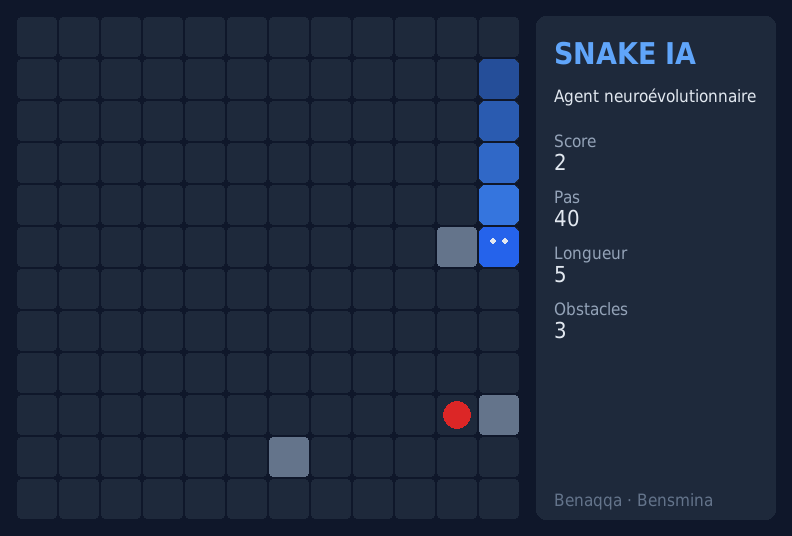
\includegraphics[width=0.62\linewidth]{demo_pygame.png}
\caption{Sortie perceptive (\emph{feedback}) : fenêtre Pygame de démonstration.
Serpent en dégradé (tête mise en évidence), nourriture, obstacles, et panneau
d'information en direct (score, pas, longueur, obstacles).}
\label{fig:pygame}
\end{figure}

\subsection{Boucle de jeu et discrétisation du temps}
Le jeu est un système dynamique exécuté par \textbf{itérations}. Le temps est
\emph{échantillonné en pas discrets} $t_0, t_1, \dots$ et l'état évolue selon une
dynamique de transition
\[
s_{t+1} = f(s_t, a_t),
\]
où $s_t$ est l'état courant et $a_t$ l'action. \textbf{Chaque appel à \texttt{step}
constitue le pas de temps discret} $t \to t+1$ : la discrétisation du temps est donc
bien présente, simplement \emph{de durée non physique}. Le jeu étant \emph{au tour
par tour} (et non en temps réel), il n'y a pas de pas de temps physique $\Delta t$
variable ni de budget de \textit{frame} à respecter : une transition par décision.
La boucle d'interaction agent–environnement s'écrit :
\begin{lstlisting}[language=Python]
obs, info = env.reset(seed=...)          # Input initial : etat de depart
done = False
while not done:                          # Boucle de jeu (par tour)
    action = agent.act(obs)              #   Decision : observation -> action
    obs, reward, terminated, truncated, info = env.step(action)  # Update + regles
    done = terminated or truncated       #   Condition d'arret
\end{lstlisting}
Ce schéma correspond au cycle \emph{Perception $\to$ Décision $\to$ Action} (PDA) :
l'agent \emph{observe} ($\texttt{obs}$), \emph{décide} ($\texttt{act}$), puis le
moteur \emph{met à jour} l'état et renvoie le \emph{feedback}.

\subsection{État global et observation locale ($o = \varphi(s)$)}
Il faut distinguer l'\textbf{état} et l'\textbf{observation}, conformément au cadre
du cours. L'\emph{état global} $s_t$ contient toute l'information nécessaire à la
simulation : positions de \emph{tout} le corps du serpent, direction courante,
ensemble des obstacles, position de la nourriture, compteur de faim et score.
L'\emph{observation} $o_t = \varphi(s_t)$ est seulement ce que l'agent perçoit : un
vecteur compact de \textbf{11~composantes}. Ce sont en pratique des
\emph{indicateurs binaires} à valeurs dans $\{0,1\}$ (l'espace est néanmoins déclaré
\texttt{Box}$(-1,1)$ pour la conformité Gymnasium et une éventuelle extension), ce
qui en fait une entrée idéale pour un contrôleur de type réseau de neurones.
\begin{center}
\begin{tabular}{cl}
\toprule
\textbf{Indices} & \textbf{Signification} \\
\midrule
0--2  & Danger immédiat (tout droit / droite / gauche) \\
3--6  & Direction courante (encodage \emph{one-hot} : haut/droite/bas/gauche) \\
7--10 & Position relative de la nourriture (gauche/droite/haut/bas) \\
\bottomrule
\end{tabular}
\end{center}
La fonction de perception $\varphi$ est donc une \emph{compression} de l'état global
en une représentation \textbf{égocentrique et locale} (« qu'est-ce qui est dangereux
autour de moi, où est la nourriture ? »). Ce choix de conception a trois vertus :
réduire la dimension d'entrée de la décision, favoriser la \emph{généralisation}
(l'agent ne mémorise pas une carte précise), et rendre le problème
\emph{partiellement observable} de façon réaliste — l'agent ne « voit » pas
l'intégralité de la grille, exactement comme une IA de jeu dotée d'un champ de
perception limité. Le revers (analysé en section~5) est que cette myopie empêche
d'anticiper les pièges à plusieurs cases.

\subsection{Espace d'actions}
L'espace d'actions est \textbf{discret} et contient 3~actions \emph{relatives}
au serpent : aller \emph{tout droit}, \emph{tourner à droite}, \emph{tourner à
gauche}. Un bon espace d'action doit être \emph{expressif} (permettre les
comportements voulus), \emph{contrôlable} (éviter l'explosion combinatoire),
\emph{aligné} avec la dynamique, et \emph{stable}. Notre choix relatif à 3~actions
satisfait ces critères : plus simple qu'un espace absolu à 4~directions, il
\textbf{élimine mécaniquement les demi-tours suicidaires} (impossibles à exprimer)
et réduit la dimension du problème, conformément au cadrage « espace d'actions
discret simple » imposé par l'énoncé.

\subsection{Règles, transition et dynamique}
Les \textbf{règles} définissent ce que « fait » la fonction de transition $f$ :
les effets des actions, les interactions (collisions), et les conditions d'arrêt.
Concrètement, à chaque \texttt{step}, le moteur : (i)~tourne la direction selon
l'action, (ii)~calcule la nouvelle tête, (iii)~teste la collision (mur, obstacle,
corps), (iv)~gère l'ingestion (croissance + nouvelle nourriture) ou l'avance
simple (retrait de la queue), (v)~vérifie la faim et la victoire.

Concernant la nature de la dynamique : la transition est \textbf{déterministe}
\emph{à l'intérieur d'un épisode} — pour un même état et une même action, le
résultat est toujours identique, ce qui garantit la reproductibilité de
l'évaluation, $P(s_{t+1}\mid s_t, a_t) \in \{0,1\}$. La \textbf{stochasticité} est
injectée uniquement au \texttt{reset} (placement aléatoire des obstacles et de la
nourriture, tirage du nombre d'obstacles), via un générateur aléatoire ensemencé
par une graine. Cette séparation est un choix d'ingénierie important : elle permet
un aléa \emph{contrôlé} et \emph{rejouable} (deux épisodes de même graine sont
identiques au pixel près), indispensable pour comparer équitablement les agents.

\subsection{Objectifs et fonction de récompense}
L'\textbf{objectif} du jeu est de maximiser le score (nourriture mangée) tout en
survivant. La \textbf{récompense} $r_t = R(s_t, a_t, s_{t+1})$ est un signal
numérique qui mesure la qualité d'un comportement ; elle combine ici l'objectif
principal et un \emph{shaping} léger :
\[
r =
\begin{cases}
+1.0 & \text{si la nourriture est mangée}, \\
-1.0 & \text{en cas de collision (mort)}, \\
-0.5 & \text{en cas de famine}, \\
+0.1 & \text{si l'agent se rapproche de la nourriture}, \\
-0.15 & \text{s'il s'en éloigne}, \\
-0.01 & \text{coût de temps par pas},
\end{cases}
\]
la victoire (grille entièrement remplie) octroyant un bonus de $+5$. Le
\emph{shaping} de distance accélère l'apprentissage en fournissant un signal dense
plutôt qu'une récompense éparse.

\paragraph{Le piège de la récompense « trichable ».} Un principe de conception
central est qu'il faut \emph{récompenser ce que l'on veut réellement obtenir}, et
non un indicateur ambigu. Deux écueils nous menaçaient : récompenser la seule
survie inciterait au \emph{camping} (l'agent ne fait rien d'utile), et récompenser
la seule proximité à la nourriture inciterait à \emph{tourner en rond} près
d'elle. Nous mitigeons ces dérives par le faible \textbf{coût de temps} par pas
(qui pénalise les boucles stériles) et surtout par la \textbf{domination du score}
($\times 100$) dans la fitness évolutionnaire (section~3.3), de sorte que la survie
ne soit qu'un bonus secondaire.

\subsection{Conditions de fin et conformité à l'API Gymnasium}
L'environnement implémente strictement l'API \texttt{gymnasium.Env}. L'espace
d'actions est déclaré \texttt{spaces.Discrete(3)} et l'espace d'observations
\texttt{spaces.Box(-1, 1, shape=(11,))}. La méthode \texttt{step} renvoie le
quintuplet standard \texttt{(obs, reward, terminated, truncated, info)} : un épisode
se \emph{termine} (\texttt{terminated}) en cas de collision, de famine ou de
victoire ; il est \emph{tronqué} (\texttt{truncated}) au-delà d'un nombre maximal de
pas fixé par le protocole. Le dictionnaire \texttt{info} expose des variables d'état
utiles (score, nombre d'obstacles, cause de fin) pour l'analyse, sans servir à la
décision. Cette conformité garantit que l'environnement est interchangeable avec
n'importe quel outil de l'écosystème Gymnasium.

\subsection{Grille dynamique}
La spécificité du Sujet~2 est que les conditions varient \emph{selon les
épisodes}. À chaque \texttt{reset}, l'environnement tire aléatoirement :
\begin{itemize}[nosep]
  \item le nombre d'obstacles fixes, dans l'intervalle $[3, 10]$ ;
  \item le budget de faim, à $\pm 20\%$ de sa valeur de base $N^2$.
\end{itemize}
Les obstacles sont placés aléatoirement sur la grille (en évitant le corps initial
du serpent et la zone immédiatement devant sa tête). Cette variabilité empêche
l'agent de mémoriser une carte fixe et l'oblige à apprendre une \emph{politique
générale} robuste à la configuration — c'est l'incertitude événementielle qui
distingue un vrai jeu d'un simple programme déterministe.

% ======================= 3. AGENT ET ALGORITHME GENETIQUE ======================= %
\section{Agent et algorithme génétique}

Dans la taxonomie des agents de jeu (scripté $\to$ réactif $\to$ délibératif $\to$
adaptatif $\to$ \textbf{évolutif/apprenant}), notre agent se situe à l'extrémité
\emph{évolutive} : sa politique n'est pas codée à la main mais \emph{optimisée
hors ligne} par recherche évolutionnaire. Il s'oppose ainsi directement à notre
baseline \emph{réactive} (l'heuristique, à base de règles \texttt{si/alors}). Cette
section décrit la politique (le contrôleur $\pi$), son génome, et l'algorithme qui
le fait évoluer.

\subsection{Politique : réseau de neurones}
La politique de l'agent est un \textbf{perceptron multicouche} (MLP) :
\[
\text{obs}_{(11)} \xrightarrow{W_1, b_1} \tanh \xrightarrow{(16)} \xrightarrow{W_2, b_2} \text{logits}_{(3)} \xrightarrow{\arg\max} \text{action}.
\]
L'entrée est le vecteur d'observation (11), suivie d'une couche cachée de
16~neurones à activation $\tanh$, puis d'une couche de sortie produisant un score
par action. L'action retenue est l'\texttt{argmax} (politique \emph{déterministe},
ce qui garantit la reproductibilité de l'évaluation).

\subsection{Génome}
Le \textbf{génome} d'un individu est le vecteur aplati de tous les paramètres du
réseau :
\[
\dim(\text{génome}) = \underbrace{11\times16}_{W_1} + \underbrace{16}_{b_1}
+ \underbrace{16\times3}_{W_2} + \underbrace{3}_{b_2} = \mathbf{243}.
\]
Évoluer ces 243~réels revient à chercher la meilleure politique dans un espace
continu de dimension 243.

\subsection{Fonction de fitness}
La fitness d'un génome est évaluée sur \textbf{6~épisodes} (graines fixées au sein
d'une même génération, pour une comparaison équitable). En notant $\bar s$ le
score \emph{moyen sur ces 6~épisodes} (nourriture mangée), $\bar t$ le nombre de
pas moyen et $\bar R$ la récompense cumulée moyenne :
\[
\text{fitness} = 100\,\bar s + 0.5\,\bar t + \bar R.
\]
La nourriture domine le critère ($\times 100$), conformément à l'objectif
« maximiser score et survie » : la survie ($\bar t$) n'intervient que comme bonus
secondaire, afin d'éviter de récompenser un serpent qui survit sans jamais manger.

\subsection{Opérateurs génétiques}
\begin{description}[leftmargin=1.5cm,style=nextline,nosep]
  \item[Sélection] par \textbf{tournoi} de taille~5 : on tire 5~individus au hasard
        et on retient le meilleur. Cela maintient une pression de sélection
        modérée tout en préservant la diversité.
  \item[Croisement] \textbf{uniforme} : chaque gène de l'enfant provient
        aléatoirement de l'un des deux parents (probabilité $0.7$ d'appliquer le
        croisement, sinon clonage du premier parent).
  \item[Mutation] \textbf{gaussienne} additive : chaque gène est perturbé avec
        probabilité $0.1$ par un bruit $\mathcal{N}(0,\sigma^2)$. L'amplitude
        $\sigma$ décroît linéairement de $0.25$ à $0.10$ au fil des générations
        (exploration forte au début, affinage en fin).
  \item[Élitisme] les 12\% meilleurs individus sont copiés tels quels dans la
        génération suivante, garantissant que la meilleure solution n'est jamais
        perdue.
\end{description}

\subsection{Boucle d'évolution}
\begin{lstlisting}
for gen in range(n_generations):
    # 1. Évaluer la fitness de chaque individu (multi-épisodes)
    fitnesses = [evaluate_genome(ind, ...) for ind in population]
    # 2. Conserver les meilleurs (élitisme)
    new_pop = elites(population, fitnesses)
    # 3. Reproduire jusqu'à remplir la population
    while len(new_pop) < pop_size:
        p1, p2 = tournoi(fitnesses), tournoi(fitnesses)
        enfant = mutation(croisement(p1, p2))
        new_pop.append(enfant)
    population = new_pop
\end{lstlisting}

% ======================= 4. PROTOCOLE EXPERIMENTAL ======================= %
\section{Protocole expérimental}

\subsection{Hyperparamètres}
\begin{center}
\begin{tabular}{ll@{\hspace{2cm}}ll}
\toprule
\textbf{Paramètre} & \textbf{Valeur} & \textbf{Paramètre} & \textbf{Valeur} \\
\midrule
Taille de grille      & $12\times12$ & Taille de population  & 150 \\
Obstacles (dynamique) & $[3,10]$     & Nombre de générations & 150 \\
Couche cachée         & 16 neurones  & Fraction d'élite      & 12\,\% \\
Taille du génome      & 243          & Taille de tournoi     & 5 \\
Taux de mutation      & 0.10         & Croisement            & 0.70 \\
$\sigma$ mutation     & $0.25\to0.10$& Épisodes d'éval./ind. & 6 \\
Pas max / épisode     & 400          & Graine AG             & 42 \\
\bottomrule
\end{tabular}
\end{center}

\subsection{Baselines de comparaison}
Conformément à l'exigence d'au moins une baseline, nous en utilisons deux :
\begin{itemize}[nosep]
  \item \textbf{Agent aléatoire} : choisit une action uniformément au hasard.
        Borne inférieure de performance.
  \item \textbf{Agent heuristique} : règle programmée à la main --- parmi les
        actions sans danger immédiat (lu dans l'observation), choisir celle qui
        rapproche de la nourriture. Baseline « forte » servant de référence
        exigeante.
\end{itemize}

\subsection{Jeux de données et reproductibilité}
Point méthodologique central : les graines utilisées pour \textbf{évaluer} l'agent
final sont \emph{disjointes} de celles vues pendant l'\textbf{entraînement}. Les
épisodes de test correspondent aux graines $[900000, 900199]$, jamais rencontrées
durant l'évolution. Tous les agents (AG et baselines) sont évalués sur
\textbf{exactement les mêmes 200~épisodes de test}, ce qui garantit une
comparaison équitable et reproductible. L'ensemble des graines, hyperparamètres
et résultats est sauvegardé au format JSON.

\subsection{Indicateurs quantitatifs}
Pour chaque agent nous reportons : le score moyen et son écart-type, le score
maximal, la survie moyenne (nombre de pas), et le taux de réussite (proportion
d'épisodes avec au moins une nourriture mangée). Une étude de \textbf{robustesse}
mesure en outre le score selon une densité d'obstacles fixée ($0, 4, 8, 12$).

% ======================= 5. RESULTATS ET DISCUSSION ======================= %
\section{Résultats et discussion}

\subsection{Dynamique de l'évolution}
La figure~\ref{fig:evo} montre l'évolution de la fitness et du score au fil des
150~générations. On observe une progression nette : le score du meilleur individu
passe d'environ $0.3$ à la première génération à des pics dépassant $13$ en fin
d'évolution, tandis que le score moyen de la population progresse de
$\approx 0$ à $\approx 5$ (avec une forte variabilité d'une génération à l'autre). La meilleure fitness atteinte est de~$1707.7$.
L'entraînement complet (150~générations, population de 150 individus) ne demande
que \textbf{$\approx 400$~s sur un simple CPU} (sans GPU) --- un atout pratique
majeur de la neuroévolution, dont l'évaluation se parallélise trivialement et ne
nécessite ni rétropropagation ni accélérateur matériel.
Le bruit résiduel des courbes provient du renouvellement des graines d'évaluation
à chaque génération (chaque génération affronte des cartes différentes), ce qui
constitue une mesure de généralisation plutôt que de surapprentissage.

\begin{figure}[h]
\centering
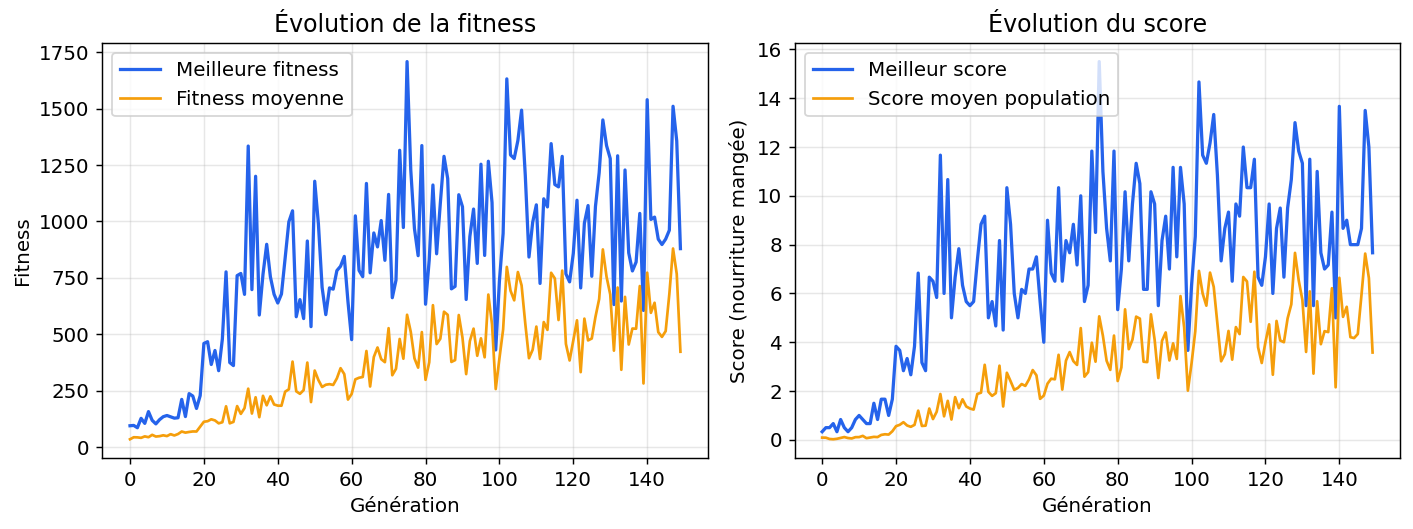
\includegraphics[width=\linewidth]{fig_evolution.png}
\caption{Évolution de la fitness (gauche) et du score (droite) au fil des
générations. Bleu : meilleur individu ; orange : moyenne de la population.}
\label{fig:evo}
\end{figure}

\subsection{Comparaison aux baselines}
Le tableau~\ref{tab:res} et la figure~\ref{fig:comp} résument les performances sur
les 200~épisodes de test indépendants.

\begin{table}[h]
\centering
\caption{Performances sur 200 épisodes de test (grille dynamique, graines
$[900000,900199]$).}
\label{tab:res}
\begin{tabular}{lccccc}
\toprule
\textbf{Agent} & \textbf{Score moy.} & \textbf{Écart-type} & \textbf{Score max}
& \textbf{Survie moy.} & \textbf{Taux succès} \\
\midrule
Aléatoire           & 0.09  & 0.30 & 2  & 15.4  & 8.5\,\% \\
AG (neuroévolution) & \textbf{6.29}  & 6.20 & 25 & \textbf{172.8} & 91.5\,\% \\
Heuristique (réf.)  & 15.97 & 6.96 & 36 & 153.1 & 100\,\% \\
\bottomrule
\end{tabular}
\end{table}

\begin{figure}[h]
\centering
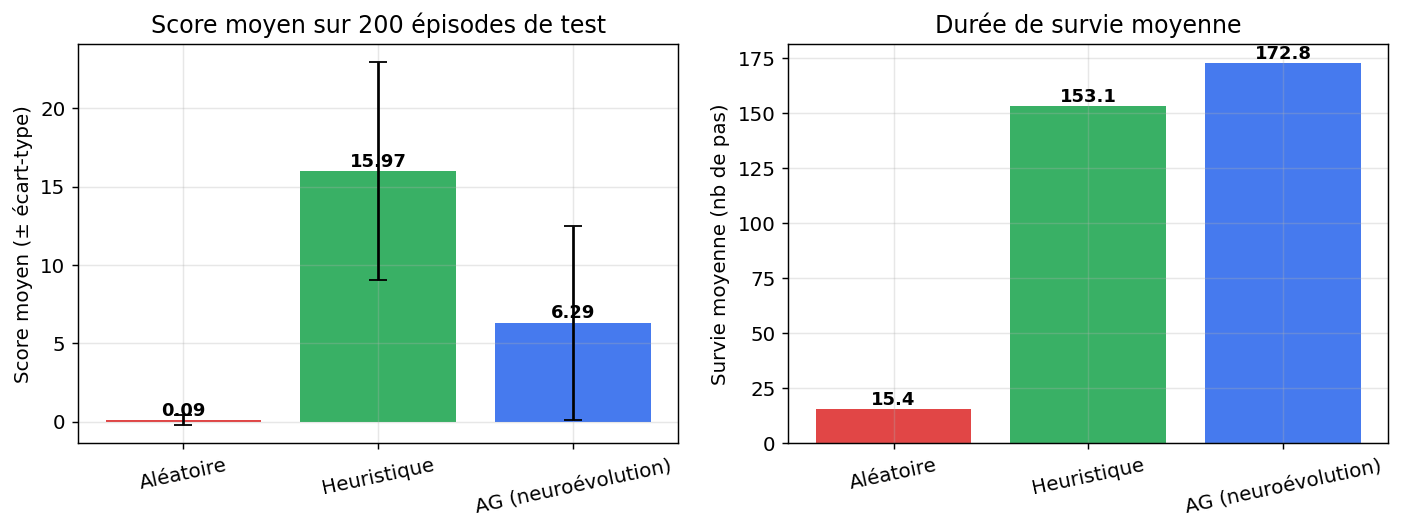
\includegraphics[width=\linewidth]{fig_comparaison.png}
\caption{Score moyen (gauche, $\pm$ écart-type) et durée de survie moyenne
(droite) des trois agents sur le jeu de test.}
\label{fig:comp}
\end{figure}

\paragraph{Interprétation.} L'agent neuroévolutionnaire améliore le score moyen
d'un facteur~$\sim70$ par rapport à l'agent aléatoire ($6.29$ contre $0.09$),
ce qui démontre sans ambiguïté que l'évolution a découvert une politique
compétente \emph{à partir de poids aléatoires}, sans aucune connaissance
programmée du jeu. Fait notable, l'agent AG \textbf{survit en moyenne plus
longtemps} que l'heuristique ($172.8$ pas contre $153.1$) : il a appris une
gestion prudente de l'espace. Il atteint un score maximal de~$25$ sur une partie.

En revanche, l'AG reste \emph{en deçà} de l'heuristique en score moyen ($6.29$
contre $15.97$). Ce résultat est attendu et instructif : l'heuristique bénéficie
d'une logique d'évitement de danger \emph{codée à la main} et toujours optimale
localement, que l'AG doit au contraire \emph{découvrir} dans un espace de 243
paramètres avec un budget limité de 150~générations.

\subsection{Distribution des scores}
La figure~\ref{fig:dist} compare les distributions de scores. L'AG présente une
distribution étalée : beaucoup d'épisodes à score faible (parties difficiles,
forte densité d'obstacles) mais une queue droite atteignant des scores élevés. La
médiane de l'AG est de~4 contre 16 pour l'heuristique.

\begin{figure}[h]
\centering
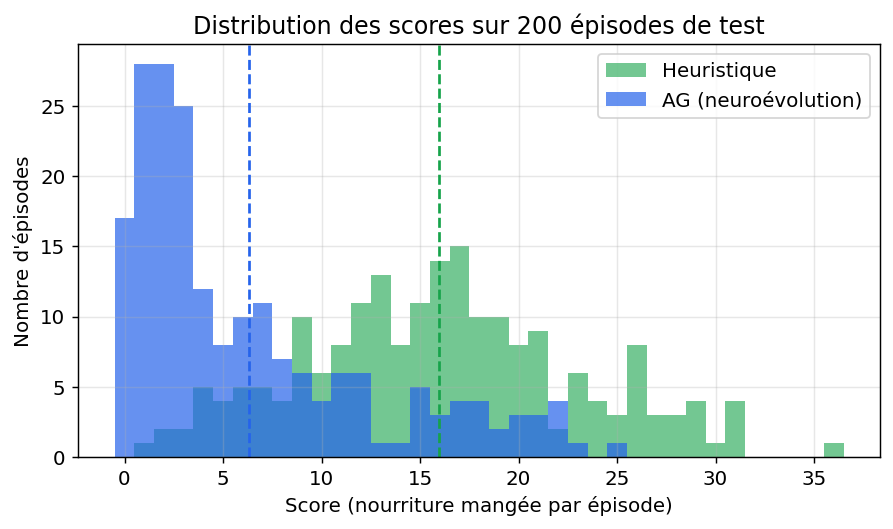
\includegraphics[width=0.78\linewidth]{fig_distribution.png}
\caption{Distribution des scores sur les 200 épisodes de test. Les lignes
pointillées indiquent les moyennes.}
\label{fig:dist}
\end{figure}

\subsection{Étude de robustesse}
La figure~\ref{fig:rob} révèle un résultat éclairant. \textbf{Sur grille sans
obstacle}, l'AG ($18.93$) rivalise presque avec l'heuristique ($19.85$) : la
politique apprise de recherche de nourriture est donc excellente. La performance
de l'AG chute cependant rapidement avec la densité d'obstacles ($9.6$ à 4
obstacles, $2.5$ à 12), beaucoup plus vite que l'heuristique. L'écart global
constaté précédemment s'explique donc essentiellement par une \textbf{gestion
sous-optimale des obstacles}, et non par une mauvaise recherche de nourriture.
Le tableau~\ref{tab:rob} détaille ces scores moyens (figure~\ref{fig:rob}).

\begin{table}[h]
\centering
\caption{Score moyen selon le nombre d'obstacles fixés (grille statique
$12\times12$, 60~épisodes par niveau).}
\label{tab:rob}
\begin{tabular}{lcccc}
\toprule
\textbf{Agent} & \textbf{0 obst.} & \textbf{4 obst.} & \textbf{8 obst.} & \textbf{12 obst.} \\
\midrule
Aléatoire           & 0.18           & 0.07          & 0.12          & 0.07 \\
AG (neuroévolution) & \textbf{18.93} & 9.60          & 4.42          & 2.52 \\
Heuristique (réf.)  & 19.85          & \textbf{18.73}& \textbf{15.38}& \textbf{11.62} \\
\bottomrule
\end{tabular}
\end{table}

\begin{figure}[h]
\centering
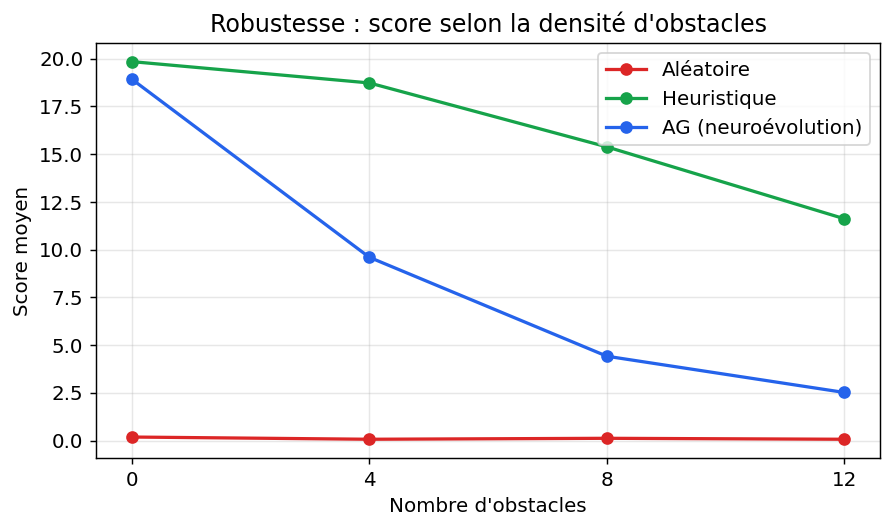
\includegraphics[width=0.78\linewidth]{fig_robustesse.png}
\caption{Score moyen selon la densité d'obstacles (grille statique). L'AG égale
presque l'heuristique sans obstacle mais se dégrade plus vite.}
\label{fig:rob}
\end{figure}

\subsection{Limites}
\begin{itemize}[nosep]
  \item \textbf{Observation locale} : la perception ne « voit » que le danger
        immédiat (une case). Le serpent ne peut pas anticiper les pièges à
        plusieurs cases ni les impasses, ce qui explique sa fragilité face aux
        obstacles denses et à son propre corps lorsqu'il s'allonge.
  \item \textbf{Coût d'évaluation} : la fitness étant bruitée (6~épisodes
        aléatoires), un bon individu peut être sous-évalué par malchance,
        ralentissant la convergence.
  \item \textbf{Capacité du réseau} : 16~neurones cachés et 243~paramètres
        limitent la complexité de la politique apprenable.
  \item \textbf{Budget évolutif} : 150~générations restent modestes pour la
        neuroévolution ; les courbes ne sont pas encore saturées.
\end{itemize}

\subsection{Pistes d'amélioration}
\begin{itemize}[nosep]
  \item \textbf{Enrichir l'observation} : ajouter une vision sur plusieurs cases
        (rayons de distance aux dangers), la longueur du serpent, ou une carte
        locale, pour permettre l'anticipation.
  \item \textbf{Réduire le bruit de fitness} : augmenter le nombre d'épisodes
        d'évaluation ou utiliser des graines communes (CRN, \emph{common random
        numbers}).
  \item \textbf{Opérateurs avancés} : mutation auto-adaptative, ou stratégies
        d'évolution modernes (CMA-ES) qui adaptent la covariance.
  \item \textbf{Topologie évolutive} (NEAT) : faire évoluer aussi la structure du
        réseau et non seulement ses poids.
  \item \textbf{Curriculum} : commencer avec peu d'obstacles puis augmenter
        progressivement la difficulté.
\end{itemize}

% ======================= 6. CONCLUSION ======================= %
\section{Conclusion}

Nous avons conçu, de bout en bout, un environnement Gymnasium personnalisé pour
une variante \emph{dynamique} du jeu Snake (Sujet~2), puis un agent
neuroévolutionnaire dont les 243~poids d'un MLP sont optimisés par un algorithme
génétique complet (sélection par tournoi, croisement uniforme, mutation gaussienne
à amplitude décroissante, élitisme). Le protocole expérimental, reproductible et
fondé sur une séparation stricte entre épisodes d'entraînement et de test, montre
que l'agent évolué apprend une politique nettement supérieure au hasard (score
moyen $\times 70$) et survit même plus longtemps que la baseline heuristique.

L'analyse critique met en évidence que l'écart résiduel avec l'heuristique provient
surtout d'une gestion perfectible des obstacles, conséquence directe d'une
observation purement locale --- un diagnostic confirmé par l'étude de robustesse,
où l'agent égale presque l'heuristique en l'absence d'obstacle. Ces limites
ouvrent des pistes d'amélioration concrètes (perception enrichie, réduction du
bruit de fitness, stratégies d'évolution avancées, curriculum), qui constitueraient
la suite naturelle de ce travail.

Au-delà des chiffres, ce projet illustre l'intérêt de la neuroévolution comme
alternative sans gradient pour l'apprentissage de comportements de jeu : à partir
d'une initialisation purement aléatoire et sans aucune connaissance experte
injectée, l'évolution fait émerger une stratégie cohérente de recherche de
nourriture et de survie.

\vspace{1cm}
\noindent\rule{\linewidth}{0.4pt}\\
{\footnotesize \textbf{Reproductibilité.} Tout le code (environnement, agents,
algorithme génétique, scripts d'entraînement et de figures) est fourni dans
l'archive du projet. L'expérience complète se relance par
\texttt{python experiments/train.py} puis \texttt{python experiments/make\_figures.py}.}

\end{document}
